\chapter{Experimento}
\label{cap:experimento}
Este capítulo descreve o experimento visando avaliar a eficácia, em termos de precisão, revocação e medida-f \cite{goutte2005probabilistic}. Dessa forma,  o experimento compara a proposta com os resultados apresentados na edição de 2016 do OAEI para as ferramentas AML e RiMOM-2016.
O capítulo está dividido em três seções: planejamento, execução e análise dos dados. 

\section{Planejamento do experimento}

Nesta seção, será detalhado o planejamento do experimento que foi projetado para este trabalho. Dentro do planejamento, encontra-se a definição da questão de pesquisa e derivação de hipóteses, a seleção das variáveis dependentes e independentes, a identificação da unidade experimental e a seleção do modelo experimental que será utilizado.

O experimento adotado é do tipo comparativo, no qual será comparada a ferramenta proposta com as ferramentas AML e RiMOM-2016. O contexto do experimento é acadêmico, posto que foi executado em um laboratório, mas algoritmos com dados reais. Nas próximas subseções, o planejamento do experimento será descrito.

\subsection{Hipóteses de pesquisa}

Como mencionado no início deste capítulo, este experimento visa avaliar a proposta com relação às métricas precisão, revocação e medida-f. Levando em consideração as questões de pesquisa a seguir:

\textbf{Q1} Existe diferença na eficácia entre AML, RiMOM-2016 e a solução proposta? Se sim, qual abordagem foi melhor?
A questão de pesquisa acima implica nas seguintes hipóteses de pesquisa:

\begin{itemize}
\item H1-0: A precisão apresentada pelas abordagens é igual.
\item H1-1: A precisão entre apresentada pelas abordagens é diferente.
\item H2-0: A revocação apresentada pelas abordagens é igual.
\item H2-1: A revocação apresentada pelas abordagens é diferente.
\item H3-0: A medida-f apresentada pelas abordagens é igual.
\item H3-1: A medida-f apresentada pelas abordagens é diferente.
\end{itemize}

Caso a hipótese nula seja refutada (indicando diferença), uma análise das métricas será executada para que se possa concluir qual ferramenta se saiu melhor.
A tabela \ref{tab:hypothesis} define formalmente as hipóteses de pesquisa supracitadas. P, R e F são funções que retornam, respectivamente a precisão, revocação e medida-f, com relação às abordagens F1 (AML), F2 (RiMOM-2016) e F3 (Proposta).

\begin{table}[h]
\centering
\caption{Formalização das hipóteses}
\label{tab:hypothesis}
\begin{tabular}{|c|c|c|}
\hline
Hipótese & Hipótese Nula & Hipótese Alternativa \\ \hline
H1       & H1-0:$ P(F1) = P(F2) = P(F3) $ & H1-1:$ P(F1) \not= P(F2) \not= P(F3) $                    \\ \hline
H2       & H2-0:$ R(F1) = R(F2) = R(F3) $ & H2-1:$ R(F1) \not= R(F2) \not= R(F3) $                    \\ \hline
H3       & H3-0:$ F(F1) = F(F2) = F(F3) $ & H3-1:$ F(F1) \not= F(F2) \not= F(F3) $                    \\ \hline
\end{tabular}
\end{table}

\subsection{Seleção de Variáveis}
Seguindo o planejamento, é necessário definir as variáveis contidas no experimento. Primeiro, as variáveis independentes, também chamadas de fatores, serão apresentadas. Logo em seguida, as variáveis dependentes, no caso as métricas, serão detalhadas.

As variáveis independentes são as seguintes:
\begin{itemize}
\item \textbf{Ferramenta} : Esta variável especifica qual a ferramenta de alinhamento será avaliada
\end{itemize}

Os fatores, também conhecidos como variáveis, podem de dois tipos: independentes e dependentes. Os fatores independentes são aqueles que queremos controlar. Além disso, um fator pode conter níveis, que caracteriza a variação. Neste experimento contamos com três níveis para o fator ou variável independente que são: F1 (AML), F2(RiMOM-2016) e F3(Proposta).

Os níveis de fatores, que são  apresentados acima serão definidos na tabela \ref{tab:factor_levels}. As variáveis dependentes (métricas) são definidas abaixo:

\begin{itemize}
\item \textbf{Precisão} (P): Esta variável representa a precisão para cada um dos níveis avaliados. A definição formal para esta métrica é descrita pela equação abaixo:

\begin{equation}
P = \dfrac{|{A}\cap{B}|}{|A|}
\end{equation}

\item \textbf{Revocação} (R): Esta variável representa o recall para cada um dos níveis avaliados. A definição formal para esta métrica é descrita pela equação abaixo:

\begin{equation}
R = \dfrac{|{A}\cap{B}|}{|B|}
\end{equation}

\item \textbf{Medida-f} (F): Esta variável representa o f-measure para cada um dos níveis avaliados. A definição formal para esta métrica é descrita pela equação abaixo:

\begin{equation}
F = \dfrac{{2}\cdot{P}\cdot{R}}{P+R}
\end{equation}

\end{itemize}

\begin{table}[]
\centering
\caption{Níveis de fatores}
\label{tab:factor_levels}
\begin{tabular}{|c|c|c|}
\hline
\textbf{Fator}              & \textbf{Nível} & \textbf{Descrição}    \\ \hline
\multirow{3}{*}{Ferramenta} & F1             & Ferramenta RiMOM-2015 \\ \cline{2-3} 
                            & F2             & Ferramenta RiMOM-2016     \\ \cline{2-3} 
                            & F3             & Proprosta             \\ \hline
\end{tabular}
\end{table}

\subsection{Unidades de Experimento}
A unidade experimental deste estudo foi fornecido pela OAEI. O \textit{dataset}\footnote{\url{http://islab.di.unimi.it/content/im_oaei/2016/\#doremus}} é composto por três variações (9-heterogeneities,4-heterogeneities e falsepositives-trap). Cada uma das variações conta com um alinhamento de referência, para que seja possível calcular as métricas.

Devido a problemas durante a execução, foram avaliadas apenas duas variações. A tabela \ref{tab:cenarios} apresenta os cenários. Vale a pensa ressaltar que não há a necessidade de cenários em que um \textit{dataset} é alinhado com ele mesmo, pois não há recursos duplicados nos \textit{datasets}. Além disso, não há a necessidade de criar cenário em que haja a permutação entre os \textit{datasets}.

\begin{table}[h]
\centering
\caption{Cenários de alinhamento}
\label{tab:cenarios}
\begin{tabular}{|c|c|}
\hline
\textbf{Cenário} & \textbf{Datasets}          \\ \hline
C1               & 9-heterogeneities          \\ \hline
C2               & falsepositives-trap        \\ \hline
\end{tabular}
\end{table}

Para este experimento, com exceção dos dados fornecidos pela dbpedia, os demais foram transformados para RDF através da ferramenta OpenRefine e persistidos no Virtuoso.  
Todo o experimento foi executado utilizando a entidade City como conceito principal. A escolha desse conceito se deve ao fato deste ser o principal conceito.

\subsection{Seleção do Projeto Experimental}
Levando em consideração as diversas classificações de experimento \cite{montgomery2012design}, o presente experimento é classificado como fatorial completo com blocagem. A blocagem foi escolhida com o objetivo de suprimir os efeitos dos \textit{datasets} nas variáveis resposta. Para cada cenário houve a execução de todos os níveis de fatores, garantindo a completude do experimento. Dessa forma temos 2 cenários possíveis, com 3 execuções em cada um deles, totalizando 6 execuções.

\section{Execução do experimento}
Esta seção descreve a execução do experimento que foi planejado na seção anterior, ou seja, descreve quais instrumentos foram utilizados, bem como a narrativa de execução do experimento.

\subsection{Preparação e instrumentação}
Inicialmente é necessário preparar o ambiente em que os alinhamentos serão executados. As ferramentas utilizadas, bem como suas versões são descritas a seguir:

\begin{itemize}
\item Virtuoso RDF Store - 07.20.3217;
\item Python - 2.7;
\item OpenJDK 64-Bit Server VM (build 25.111-b14, mixed mode)

\end{itemize}

Para isolar os efeitos entre as execuções, todo o experimento foi conduzido em um container, que permite isolar as aplicações, fazendo com que as aplicações sejam executadas em ambientes idênticos.

\subsection{Narrativa do experimento}
A Figura \ref{fig:experiment} apresenta os passos de execução de cada alinhamento, que são descritos abaixo:
\begin{itemize}
\item Construir container com as configurações zeradas;
\item Carregar dos dados;
\item Executar ferramenta dentro do container;
\item Coletar dados de alinhamento;
\item Destruir container;
\item Analisar dados;
\end{itemize}

\begin{figure}[h]
	\centering
	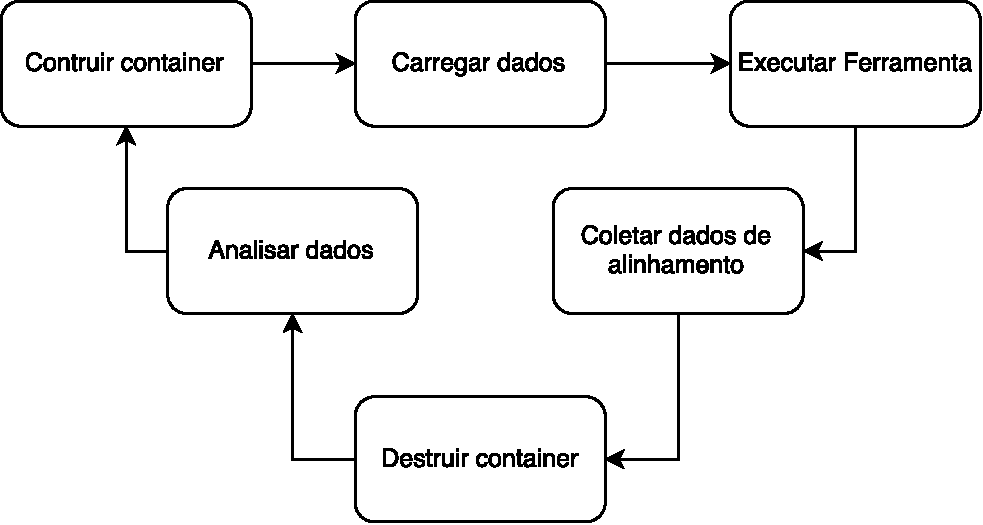
\includegraphics[width=0.9\textwidth]{./imagens/experimento.pdf}
    \caption{Processo de execução do experimento}
	\label{fig:experiment}
\end{figure}

\subsection{Análise de Ameaças à Validade}
Embora todo experimento tenha sido projetado para minimizar possíveis ameaças que comprometam suas conclusões, existem algumas ameaças que devem ser mencionadas. Uma possível ameaça à validade do experimento é com relação a quantidade de amostras, o número de recursos, bem como a quantidade de \textit{datasets} pode influenciar o resultado do alinhamento.
Levando isso em consideração, na próxima seção, os dados obtidos a partir da execução do experimento serão analisados.

\subsection{Análise dos dados}
O experimento foi conduzido de acordo com o planejamento descrito anteriormente neste capítulo, depois da execução, os \textit{datasets} de alinhamento eram coletados. Os dados de precisão, revocação e medida-f eram calculados de acordo com as funções especificadas anteriormente.
Ao longo desta seção, uma análise descritiva dos dados obtidos será conduzida, envolve, a apresentação das métricas referentes a cada cenário.

As figuras \ref{fig:cenario1}, \ref{fig:cenario2} apresentam as ferramentas de acordo com seus resultados em cada um dos cenários. A Tabela \ref{tab:resultados} sumariza os dados obtidos para cada cenário.

\begin{table}[h]
	\centering
	\caption{Sumarização dos dados relativos a precisão, revocação e medida-f por cenário.}
	\label{tab:resultados}
	\begin{tabular}{|c|c|c|c|c|}
		\hline
		      Cenário       & Ferramenta & Precisão & Revocação & Medida-F \\ \hline
		\multirow{3}{*}{C1} &  Proposta  &    1     &   0.875   &  0.933   \\ \cline{2-5}
		                    &    AML     &  0.966   &   0.875   &  0.918   \\ \cline{2-5}
		                    &   RiMOM    &  0.813   &   0.813   &  0.813   \\ \hline
		\multirow{3}{*}{C2} &    AML     &  0.921   &   0.854   &  0.886   \\ \cline{2-5}
		                    &  Proposta  &  0.906   &   0.707   &  0.794   \\ \cline{2-5}
		                    &   RiMOM    &  0.707   &   0.707   &  0.707   \\ \hline
	\end{tabular}
\end{table}

\begin{center}
\begin{figure}
	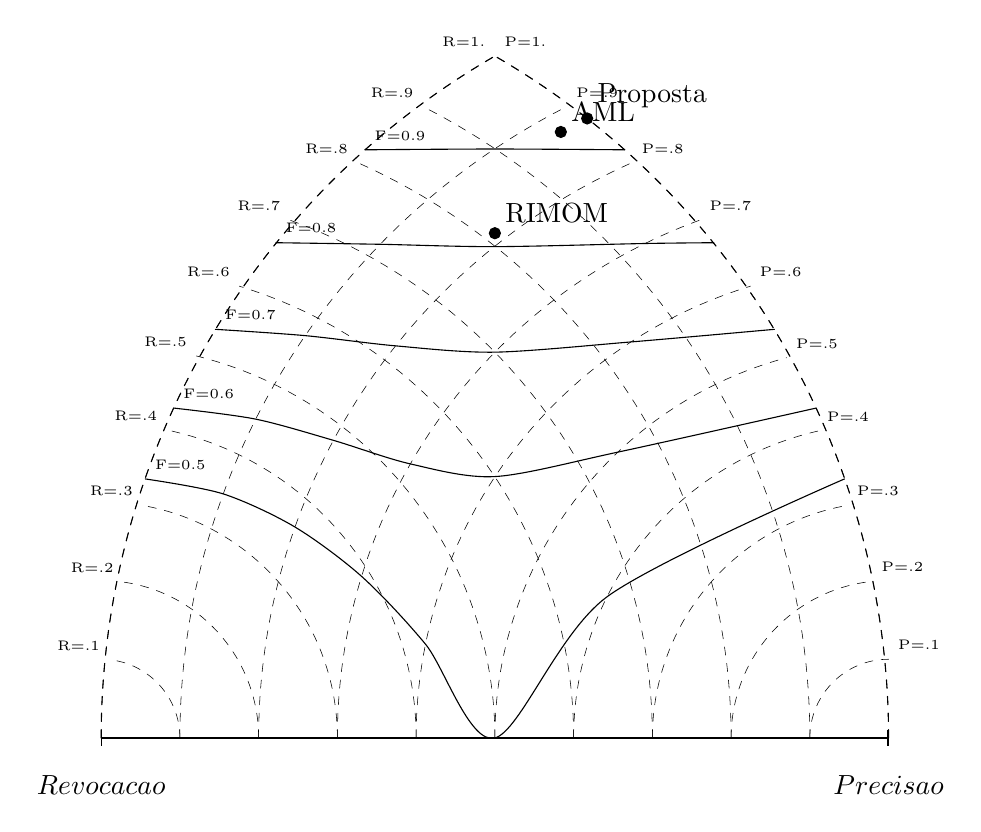
\begin{tikzpicture}[cap=round]{H}
	%\draw[step=1cm,very thin,color=gray] (0,0) grid (10.0,9.0);
	\draw[|-|] (-0,0) -- (10,0);
	\draw[dashed,very thin] (10,0) arc (0:60:10cm);
	\draw[dashed,very thin] (0,0) arc (180:120:10cm);
	\draw[dashed] (10,0) arc (0:60:10cm) node[anchor=south east]  {{\tiny R=1.}};
	\draw[dashed,very thin] (9,0) arc (0:63:9cm) node[anchor=south east] {{\tiny R=.9}};
	\draw[dashed,very thin] (8,0) arc (0:66:8cm) node[anchor=south east]  {{\tiny R=.8}};
	\draw[dashed,very thin] (7,0) arc (0:70:7cm) node[anchor=south east]  {{\tiny R=.7}};
	\draw[dashed,very thin] (6,0) arc (0:73:6cm) node[anchor=south east]  {{\tiny R=.6}};
	\draw[dashed,very thin] (5,0) arc (0:76:5cm) node[anchor=south east] {{\tiny R=.5}};
	\draw[dashed,very thin] (4,0) arc (0:78:4cm) node[anchor=south east] {{\tiny R=.4}};
	\draw[dashed,very thin] (3,0) arc (0:80:3cm) node[anchor=south east] {{\tiny R=.3}};
	\draw[dashed,very thin] (2,0) arc (0:82:2cm) node[anchor=south east] {{\tiny R=.2}};
	\draw[dashed,very thin] (1,0) arc (0:84:1cm) node[anchor=south east] {{\tiny R=.1}};
	\draw[dashed] (0,0) arc (180:120:10cm) node[anchor=south west] {{\tiny P=1.}};
	\draw[dashed,very thin] (1,0) arc (180:117:9cm) node[anchor=south west] {{\tiny P=.9}};
	\draw[dashed,very thin] (2,0) arc (180:114:8cm) node[anchor=south west] {{\tiny P=.8}};
	\draw[dashed,very thin] (3,0) arc (180:110:7cm) node[anchor=south west] {{\tiny P=.7}};
	\draw[dashed,very thin] (4,0) arc (180:107:6cm) node[anchor=south west] {{\tiny P=.6}};
	\draw[dashed,very thin] (5,0) arc (180:105:5cm) node[anchor=south west] {{\tiny P=.5}};
	\draw[dashed,very thin] (6,0) arc (180:103:4cm) node[anchor=south west] {{\tiny P=.4}};
	\draw[dashed,very thin] (7,0) arc (180:100:3cm) node[anchor=south west] {{\tiny P=.3}};
	\draw[dashed,very thin] (8,0) arc (180:96:2cm) node[anchor=south west] {{\tiny P=.2}};
	\draw[dashed,very thin] (9,0) arc (180:90:1cm) node[anchor=south west] {{\tiny P=.1}};
	\draw (0.56,3.29) node[anchor=south west] {\tiny{F=0.5}};
	\draw plot[smooth] coordinates { (0.56,3.29) (1.55,3.10) (2.46,2.68) (3.31,2.05) (4.12,1.19) (5.00,0.00) (6.42,1.79) (9.44,3.29)};
	\draw (0.92,4.19) node[anchor=south west] {\tiny{F=0.6}};
	\draw plot[smooth] coordinates { (0.92,4.19) (1.96,4.05) (2.95,3.78) (3.93,3.48) (5.00,3.32) (6.56,3.63) (9.08,4.19)};
	\draw (1.45,5.19) node[anchor=south west] {\tiny{F=0.7}};
	\draw plot[smooth] coordinates { (1.45,5.19) (2.59,5.11) (3.74,4.98) (5.00,4.90) (6.73,5.03) (8.55,5.19)};
	\draw (2.22,6.29) node[anchor=south west] {\tiny{F=0.8}};
	\draw plot[smooth] coordinates { (2.22,6.29) (3.54,6.27) (5.00,6.24) (6.91,6.28) (7.78,6.29)};
	\draw (3.35,7.47) node[anchor=south west] {\tiny{F=0.9}};
	\draw plot[smooth] coordinates { (3.35,7.47) (5.00,7.48) (6.65,7.47)};
	\draw (0,-0.6) node {$Revocacao$};
	\draw (10,-0.6) node {$Precisao$};
	%\draw (-0.2,0) node {0}; 
	%\draw (10.2,0) node {1}; 
	\draw plot[mark=*,] coordinates {(6.171875,7.86816109293)};
	\draw (6.181875,7.87816109293) node[anchor=south west] {Proposta};
	\draw plot[mark=*,] coordinates {(5.837655,7.69658262484)};
	\draw (5.847655,7.70658262484) node[anchor=south west] {AML};
	\draw plot[mark=*,] coordinates {(5.0,6.41068639071)};
	\draw (5.01,6.42068639071) node[anchor=south west] {RIMOM};
	\end{tikzpicture}
	\caption{Resultado das ferramentas para o cenário 1}
	\label{fig:cenario1}
\end{figure}
\begin{figure}
		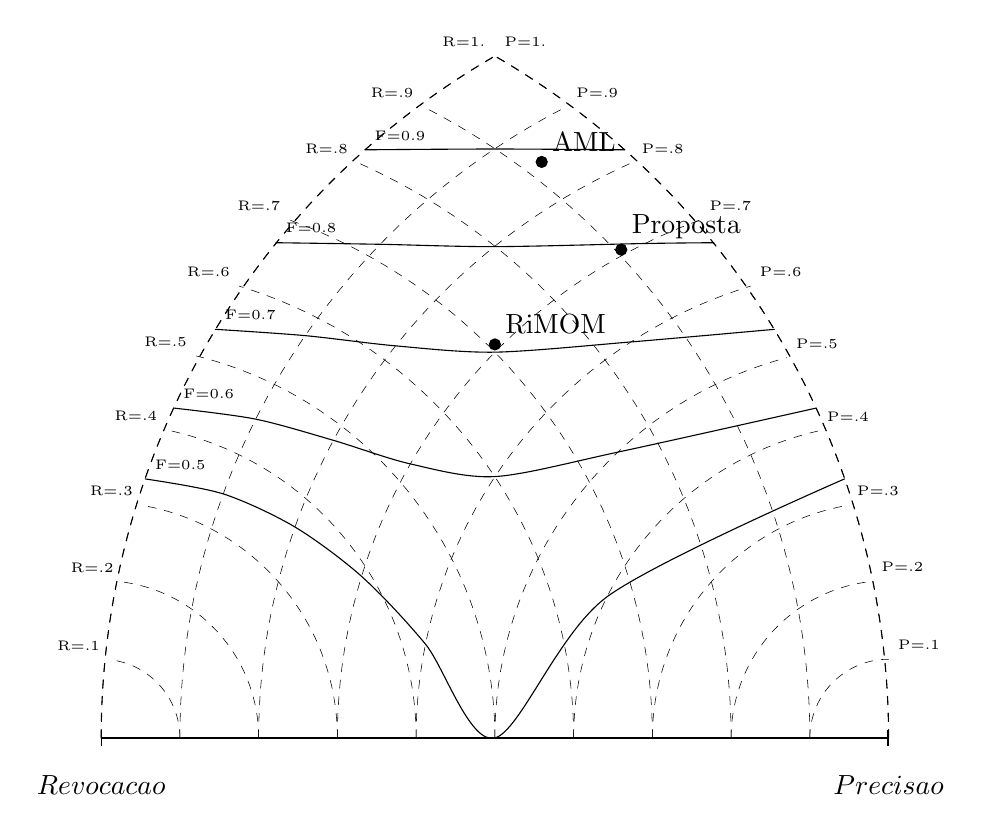
\begin{tikzpicture}[cap=round]{H}
		%\draw[step=1cm,very thin,color=gray] (0,0) grid (10.0,9.0);
		\draw[|-|] (-0,0) -- (10,0);
		\draw[dashed,very thin] (10,0) arc (0:60:10cm);
		\draw[dashed,very thin] (0,0) arc (180:120:10cm);
		\draw[dashed] (10,0) arc (0:60:10cm) node[anchor=south east]  {{\tiny R=1.}};
		\draw[dashed,very thin] (9,0) arc (0:63:9cm) node[anchor=south east] {{\tiny R=.9}};
		\draw[dashed,very thin] (8,0) arc (0:66:8cm) node[anchor=south east]  {{\tiny R=.8}};
		\draw[dashed,very thin] (7,0) arc (0:70:7cm) node[anchor=south east]  {{\tiny R=.7}};
		\draw[dashed,very thin] (6,0) arc (0:73:6cm) node[anchor=south east]  {{\tiny R=.6}};
		\draw[dashed,very thin] (5,0) arc (0:76:5cm) node[anchor=south east] {{\tiny R=.5}};
		\draw[dashed,very thin] (4,0) arc (0:78:4cm) node[anchor=south east] {{\tiny R=.4}};
		\draw[dashed,very thin] (3,0) arc (0:80:3cm) node[anchor=south east] {{\tiny R=.3}};
		\draw[dashed,very thin] (2,0) arc (0:82:2cm) node[anchor=south east] {{\tiny R=.2}};
		\draw[dashed,very thin] (1,0) arc (0:84:1cm) node[anchor=south east] {{\tiny R=.1}};
		\draw[dashed] (0,0) arc (180:120:10cm) node[anchor=south west] {{\tiny P=1.}};
		\draw[dashed,very thin] (1,0) arc (180:117:9cm) node[anchor=south west] {{\tiny P=.9}};
		\draw[dashed,very thin] (2,0) arc (180:114:8cm) node[anchor=south west] {{\tiny P=.8}};
		\draw[dashed,very thin] (3,0) arc (180:110:7cm) node[anchor=south west] {{\tiny P=.7}};
		\draw[dashed,very thin] (4,0) arc (180:107:6cm) node[anchor=south west] {{\tiny P=.6}};
		\draw[dashed,very thin] (5,0) arc (180:105:5cm) node[anchor=south west] {{\tiny P=.5}};
		\draw[dashed,very thin] (6,0) arc (180:103:4cm) node[anchor=south west] {{\tiny P=.4}};
		\draw[dashed,very thin] (7,0) arc (180:100:3cm) node[anchor=south west] {{\tiny P=.3}};
		\draw[dashed,very thin] (8,0) arc (180:96:2cm) node[anchor=south west] {{\tiny P=.2}};
		\draw[dashed,very thin] (9,0) arc (180:90:1cm) node[anchor=south west] {{\tiny P=.1}};
		\draw (0.56,3.29) node[anchor=south west] {\tiny{F=0.5}};
		\draw plot[smooth] coordinates { (0.56,3.29) (1.55,3.10) (2.46,2.68) (3.31,2.05) (4.12,1.19) (5.00,0.00) (6.42,1.79) (9.44,3.29)};
		\draw (0.92,4.19) node[anchor=south west] {\tiny{F=0.6}};
		\draw plot[smooth] coordinates { (0.92,4.19) (1.96,4.05) (2.95,3.78) (3.93,3.48) (5.00,3.32) (6.56,3.63) (9.08,4.19)};
		\draw (1.45,5.19) node[anchor=south west] {\tiny{F=0.7}};
		\draw plot[smooth] coordinates { (1.45,5.19) (2.59,5.11) (3.74,4.98) (5.00,4.90) (6.73,5.03) (8.55,5.19)};
		\draw (2.22,6.29) node[anchor=south west] {\tiny{F=0.8}};
		\draw plot[smooth] coordinates { (2.22,6.29) (3.54,6.27) (5.00,6.24) (6.91,6.28) (7.78,6.29)};
		\draw (3.35,7.47) node[anchor=south west] {\tiny{F=0.9}};
		\draw plot[smooth] coordinates { (3.35,7.47) (5.00,7.48) (6.65,7.47)};
		\draw (0,-0.6) node {$Revocacao$};
		\draw (10,-0.6) node {$Precisao$};
		%\draw (-0.2,0) node {0}; 
		%\draw (10.2,0) node {1}; 
		\draw plot[mark=*,] coordinates {(6.604935,6.20148640616)};
		\draw (6.614935,6.21148640616) node[anchor=south west] {Proposta};
		\draw plot[mark=*,] coordinates {(5.0,4.99848977192)};
		\draw (5.01,5.00848977192) node[anchor=south west] {RiMOM};
		\draw plot[mark=*,] coordinates {(5.594625,7.31602836991)};
		\draw (5.604625,7.32602836991) node[anchor=south west] {AML};
		\end{tikzpicture}
		\caption{Resultado das ferramentas para o cenário 2}
		\label{fig:cenario2}
\end{figure}
\end{center}

\subsection{Verificação das hipóteses}
Esta seção tem como objetivo validar ou refutar as hipóteses propostas. A primeira hipótese a ser verificada será feita com relação à precisão. As hipóteses nula e alternativa estão numeradas abaixo, respectivamente:
on
\begin{itemize}
\item \textbf{H1-0:} A precisão apresentada pelas abordagens é igual.
\item \textbf{H1-1:} A precisão apresentada pelas abordagens é diferente.
\end{itemize}

Para realizar a análise, devemos observar a precisão nos dois cenários de alinhamento. Como descrito na Tabela \ref{tab:resultados}, a proposta apresentou precisão de 1 para o cenário 1 e 0.906 para o cenário 2, refutando a hipótese nula (H1-0).

A próxima validação de hipótese ocorrerá com relação à revocação. As hipóteses nula e alternativa estão numeradas abaixo, respectivamente:

\begin{itemize}
\item \textbf{H2-0:} A revocação apresentada pelas abordagens é igual.
\item \textbf{H2-1:} A revocação apresentada pelas abordagens é diferente.
\end{itemize}

Diante do resultado apresentado pelas ferramentas nos dois cenários de alinhamento, onde apresentou uma revocação de 0.875 para o cenário 1 e 0.707 para o cenário 2. Apesar do bom desempenho, a proposta apresentou valores iguais a pelo menos uma das ferramentas em cada um dos cenários. Dessa forma, não é possível refutar a hipótese nula (H2-0).

Finalizando a verificação de hipóteses, serão analisadas as hipóteses relacionadas à medida-f.As hipóteses nula e alternativa estão numeradas abaixo, respectivamente:

\begin{itemize}
\item \textbf{H3-0:} A medida-f apresentada pelas abordagens é igual.
\item \textbf{H3-1:} A medida-f apresentada pelas abordagens é diferente.
\end{itemize}

Conforme os resultados apresentados na Tabela \ref{tab:resultados}, a proposta ficou em primeiro posição no cenário 1 com uma dedida-f de 0.933 e segundo lugar no cenário 2 com 0.794.


\subsection{Principais conclusões}
O experimento conduzido neste capítulo, visou avaliar a eficácia das ferramentas de alinhamento de dados conectados com relação às métricas de precisão, revocação e medida-f. Essas variáveis foram avaliadas separadamente em cada um dos dois cenários de alinhamento (9-heterogeneities e falsepositives-trap).

Pelas análises realizadas, foi possível verificar que a proposta apresentou bons resultados mesmo não utilizando abordagens dedicadas ao dataset.